\chapter{Research Methodology}

\section{Data Preparation}

We obtained our dataset from Motional AD Inc's publicly available nuScenes dataset version 1.0-mini. This dataset consists of 10 different scenes,
each approximately 20 seconds long, with annotated data provided every half a second (2 Hz).

Next, we used nuScenes devkit package in Python. This package provides a suite of tools to 
easily query and retrieve data from the nuScenes dataset. Only the front-facing camera channel (CAM\_FRONT) was utilized
with 14 classes, including drivable area, ped crossing, walkway, carpark, car, truck, bus, trailer, construction vehicle, pedestrian, motorcycle, bicycle, traffic cone, and barrier.


\section{Data Generation}
The labels or ground truth for each class are generated for training.
To generate labels, annotation data that refers to any bounding box defining the position of an object seen in a sample is required. Bounding boxes, see figure \ref{fig:BoundingBox} for an example, are projected only in x and z axis to locate 2D object position on global coordinate system.


\begin{figure}[H]
  \centering
  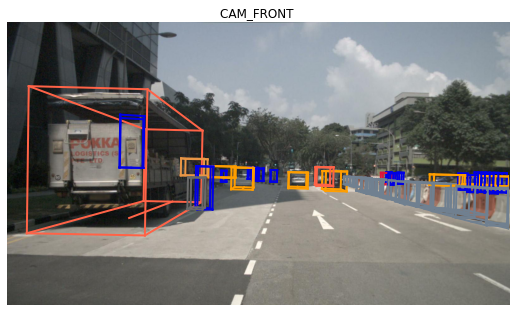
\includegraphics[width=0.75\textwidth]{img/3-bounding-box.png}
  \caption{Object bounding box}
  \label{fig:BoundingBox}
\end{figure}

Additionally, a occlusion mask is calculated. It is a mask indicating the visible view captured by a camera.
After the process, a stack of labels and mask is generated. Each layer represents as binary with respect to 14 classes and a mask. See figure \ref{fig:GeneratedLabels}.

\begin{figure}[H]
  \centering
  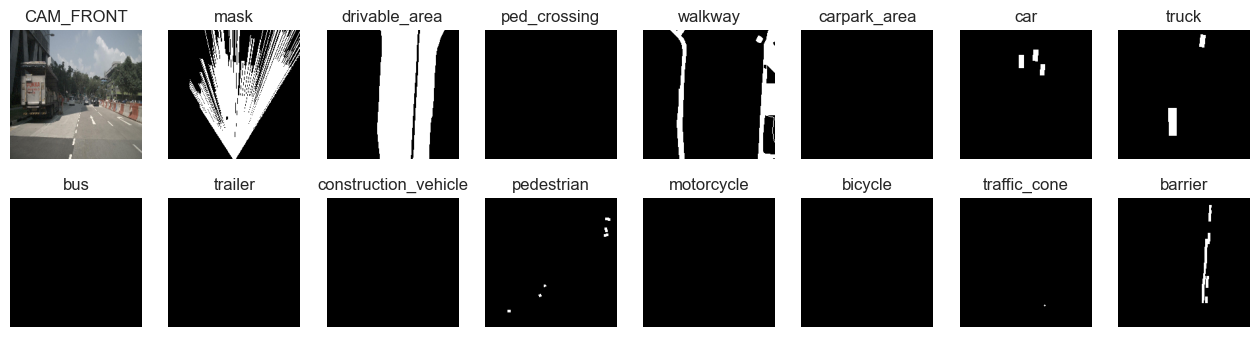
\includegraphics[width=1\textwidth]{img/3-binary-gt.png}
  \caption{Generated labels}
  \label{fig:GeneratedLabels}
\end{figure}

  
